\apendice{Plan de Proyecto Software}

\section{Introducción}
En este primer anexo se ofrece la planificación temporal seguida a lo largo del proyecto, así como una planificación del coste que conlleva el prototipo realizado. Por último se analizará la viabilidad legal contemplando las leyes pertinentes para el desarrollo de este proyecto.


\section{Planificación temporal}

En este apartado se va a recoger la información relativa a la planificación temporal del proyecto. Se ha empleado GitHub para la organización del proyecto, a través de \textit{Issues} específicas. Para etiquetar las tareas se han usado diferentes \textit{labels} que describen en qué consiste cada tarea. Todo esto lo podemos ver en este \href{https://github.com/CeliaValladolid/TFG_Valvula_Derivacion_VentriculoPeritoneal}{Repositorio}.
A continuación, en la Figura \ref{fig:planificación} podemos observar la planificación seguida y distribuida por semanas.
\begin{figure}[h]
    \centering
    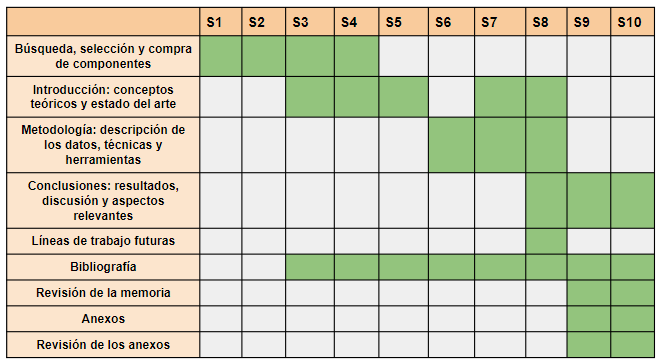
\includegraphics[width=1.1\textwidth]{img/planificacion.PNG}
    \caption{Planificación temporal. Imagen propia}
    \label{fig:planificación}
\end{figure}

\subsection{Planificación económica}

La evaluación del coste asociado a este proyecto se puede desglosar en tres partes, por un lado el gasto en hardware, por otro el gasto en software y por último el gasto personal, el gasto que conlleva sacar adelante este trabajo.

\subsubsection{Coste hardware}
Como elemento principal se necesita un ordenador, en mi caso es un Asus bastante antiguo pero si hoy en día tuviésemos que comprar uno, necesitaríamos aproximadamente unos 600€ tirando por lo bajo.

En cuanto a los componentes electrónicos:
\begin{itemize}
    \item Placa Arduino Uno R3 \cite{compraplaca}: 29,04€
    \item ProtoBoard \cite{compraproto}: 5,49€
    \item Cableado \cite{compracables}: 9,98€
    \item Cable USB \cite{comprausb}: 3,96€
    \item Sensor de presión NXP MPX5010DP \cite{comprasensor}: 22,01€ + 7,77€ (IVA) + 14,99€ (gastos de envío) = 44,77€
    \item Mini bomba \cite{comprabomba}: 7,59€ (2 ud)
    \item Relé \cite{comprarele}: 5,49€
    \item Portapilas \cite{compraporta}: 6,50€
    \item Pilas: 2€
\end{itemize}
En la siguiente tabla \ref{tab:costes} podemos ver la suma total de todo el hardware necesario.

\begin{table}[h!]
\centering
\begin{tabular}{ |c|c| }
\hline
\rowcolor[HTML]{B0E0E6} 
\textbf{Componente} & \textbf{Coste} \\
\hline
Ordenador ASUS & 600€ \\
\hline
Placa Arduino Uno R3 & 29,04€ \\
\hline
ProtoBoard & 5,49€ \\
\hline
Cableado & 9,98€ \\
\hline
Cable USB & 3,96€ \\
\hline
Sensor de presión NXP MPX5010DP & 44,77€ \\
\hline
Mini bomba & 3,79€ \\
\hline
Relé & 5,49€ \\
\hline
Portapilas & 6,50€ \\
\hline
Pilas & 2€ \\
\hline
Tubo para el sensor & 1€ \\
\hline
\rowcolor[HTML]{4682B4} 
\textbf{Total} & \textbf{712,02€} \\
\hline
\end{tabular}
\caption{Resumen de costes de hardware}
\label{tab:costes}
\end{table}

\subsubsection{Coste software}
Los costes del software empleado para elaborar el proyecto han sido nulos debido a que se han empleado aplicaciones, plataformas y entornos de código abierto en los que su uso es gratuito. 

\subsubsection{Coste de personal}
Respecto al coste de personal, vamos a suponer que el salario bruto\footnote{El salario bruto hace referencia a la cantidad de dinero que percibe el empleado antes de aplicarle las deducciones por IRPF y las cotizaciones a la Seguridad Social mientras que la cantidad total a percibir se denomina salario neto \cite{bruto}. } de un ingeniero de la salud con poca experiencia no supera los 20.000€ anuales, por lo tanto aplicando las deducciones pertinentes obtenemos las cifras recogidas en las tablas \ref{tab:costes-personal} \ref{tab:costes-personal1}.

\begin{table}[h!]
\centering
\begin{tabular}{ |c|c| }
\hline
\rowcolor[HTML]{B0E0E6} 
\textbf{Concepto} & \textbf{Coste} \\
\hline
Salario bruto anual & 20.000€ \\
\hline
Retención IRPF anual & 1.772€ \\
\hline
Cuotas a la Seguridad Social (año) & 1.349,69€ \\
\hline
\rowcolor[HTML]{4682B4} 
\textbf{Sueldo neto anual} & \textbf{16.880,31€} \\
\hline
\end{tabular}
\caption{Resumen de costes anuales de personal}
\label{tab:costes-personal}
\end{table}


\begin{table}[h!]
\centering
\begin{tabular}{ |c|c| }
\hline
\rowcolor[HTML]{B0E0E6} 
\textbf{Concepto} & \textbf{Coste} \\
\hline
Salario bruto mensual & 1.666,66€ \\
\hline
Retención IRPF mensual & 147,66€ \\
\hline
Cuotas a la Seguridad Social (mes) & 112,47€ \\
\hline
Sueldo neto mensual & 1.406,53€ \\
\rowcolor[HTML]{4682B4} 
\textbf{Sueldo total 2 meses} & \textbf{2.813,06€} \\
\hline
\end{tabular}
\caption{Resumen de costes mensuales de personal}
\label{tab:costes-personal1}
\end{table}

\subsubsection{Coste total}
El coste total para desarrollar este proyecto, supone la suma de los gastos en hardware y en personal, recogidos en la tabla \ref{tab:costes-total}.

\begin{table}[h!]
\centering
\begin{tabular}{ |c|c| }
\hline
\rowcolor[HTML]{B0E0E6} 
\textbf{Concepto} & \textbf{Coste} \\
\hline
Hardware & 712,02€ \\
\hline
Personal & 2.813,06€ \\
\rowcolor[HTML]{4682B4} 
\textbf{Total} & \textbf{3.525,08€} \\
\hline
\end{tabular}
\caption{Resumen del coste total}
\label{tab:costes-total}
\end{table}

\subsection{Viabilidad legal}
En este apartado se abordan las leyes y normativas vigentes en la actualidad que hay que tener en cuenta para el desarrollo, comercialización y posterior tratamiento de los datos personales generados.

\subsubsection{Desarrollo y comercialización del dispositivo}
En este apartado se detallan las principales leyes, normativas y normas españolas y europeas encargadas de la regulación de los diferentes productos sanitarios y la protección de las invenciones en el campo de la tecnología médica.


La \textbf{Ley 24/2015}, más conocida como la Ley de Patentes \cite{patentes}, es la responsable de regular todo lo relacionado con la protección de invenciones a través de patentes, incluyendo aspectos como su registro, derecho a la patente y todos los procedimientos indispensables para poder solicitar una patente. Asimismo, el \textbf{Real Decreto Legislativo 1/1996}, relativo a la Ley de Propiedad Intelectual \cite{propintec}, es el encargado de regular la protección del derecho de autor y derechos semejantes.

En cuanto a los productos sanitarios, están regidos por la Agencia Española de Medicamentos y Productos Sanitarios (AEMPS). Destacan principalmente dos:
\begin{enumerate}
    \item \textbf{Real Decreto 437/2002} \cite{licencias}: regula todos los aspectos relacionados con los productos sanitarios, desde su desarrollo hasta su posterior comercialización.
    \item \textbf{Real Decreto 1591/2009} \cite{prod}: regula la concesión de las diferentes licencias necesarias para la fabricación y desarrollo del producto.
\end{enumerate}

En lo que respecta a los dispositivos que serán alojados en el interior del cuerpo humano, es fundamental el empleo de materiales biocompatibles. Este punto no afecta al prototipo desarrollado a lo largo del proyecto, pero sí que es un punto a tener en cuenta en el futuro, ya que la idea es desarrollar un dispositivo implantable en el interior del cráneo. Para ello, los materiales empleados deben ser compatibles con el tejido humano y no provocar ningún tipo de rechazo. Los dispositivos médicos implantables deben ser sometidos a rigurosos controles tales como pruebas de biocompatibilidad, estudios de toxicidad, y ensayos clínicos antes de su aprobación, con el objetivo de garantizar la eficacia y la seguridad del dispositivo y del paciente. 

La norma \textbf{ISO 10993-9:2022 - Evaluación Biológica de Productos Sanitarios} \cite{norma} es la encargada de regular la biocompatibilidad de los materiales utilizados para el desarrollo de los productos. Consta de una serie de normas internacionales que establecen distintos métodos para evaluar la seguridad de los materiales.


\subsubsection{Protección de datos personales}
En un proyecto que maneja datos sensibles de pacientes, es esencial incluir un apartado dedicado a la protección de estos datos para garantizar la privacidad de los individuos y el cumplimiento de las diferentes normativas legales vigentes. La protección de datos personales en el campo de la salud  está regulada por leyes y normativas tales como el \textbf{Reglamento General de Protección de Datos (RGPD)} o \textbf{Reglamento (UE) 2016/679} en la Unión Europea y la \textbf{Ley Orgánica 3/2018, de 5 de diciembre, de Protección de Datos Personales y garantía de los derechos digitales} en España. Estas leyes establecen principios fundamentales para el tratamiento de datos, como la licitud, exactitud, transparencia, integridad y confidencialidad así como la limitación tanto de la finalidad como del plazo de conservación y la minimización de datos .
\begin{itemize}
    \item El RGPD (Reglamento (UE) 2016/679) \cite{reglaue} establece los siguientes principios relativos al tratamiento de los datos recogidos:
    \begin{enumerate}
        \item \textbf{Tratados de manera lícita, leal y transparente} (Artículo 5.1.a): la recogida de los datos debe realizarse de forma justa y transparente, informando al individuo del posterior uso que recibirán sus datos.
        \item \textbf{Recogidos con fines determinados, explícitos y legítimos}(Artículo 5.1.b): los datos únicamente pueden ser empleados para los fines para los que fueron recogidos inicialmente.
        \item \textbf{Adecuados, pertinentes y limitados a lo necesario en relación con los fines para los que son tratados} (Artículo 5.1.c): solo se deben recoger los datos estrictamente necesarios para lograr el cumplimiento de los diferentes fines.
        \item \textbf{Exactos y, si fuera necesario, actualizados} (Artículo 5.1.d): se deben adoptar medidas razonables para garantizar que los datos inexactos con respecto a los fines se supriman o rectifiquen.
        \item \textbf{Mantenidos de forma que se permita la identificación de los interesados durante no más tiempo del necesario} (Artículo 5.1.e): los datos sólo deben ser conservados durante el tiempo necesario.
        \item \textbf{Tratados de tal manera que se garantice una seguridad adecuada de los datos personales} (Artículo 5.1.f): se deben implementar las medidas técnicas y organizativas pertinentes para proteger los datos contra su pérdida, destrucción, daño accidental o contra el tratamiento no autorizado o ilícito.
    \end{enumerate}
\end{itemize}
\begin{itemize}
    \item Por otra parte, la Ley Orgánica 3/2018, de 5 de diciembre, de Protección de Datos Personales y garantía de los derechos digitales \cite{leyorgdat} incluye algunos puntos adicionales, como:
    \begin{enumerate}
        \item \textbf{Tratamiento basado en el consentimiento del afectado} (Artículo 6): sólo será lícito el tratamiento de datos personales si el interesado  da su consentimiento inequívoco para una o varias finalidades. Por consentimiento se entiende toda manifestación de voluntad libre, específica, informada e inequívoca por la que este acepta el tratamiento de sus datos personales. Se debe asegurar que el afectado acepta y entiende las condiciones bajo las que sus datos serán tratados.
        \item \textbf{Derechos de los afectados} (Artículos 13-18): los individuos tienen derecho a acceder (13), rectificar (14), suprimir (15), limitar el tratamiento (16), solicitar la portabilidad (17) y oponerse (18) al tratamiento de los datos.
    \end{enumerate}
\end{itemize}

Uno de los aspectos más importantes cuando se trabaja con datos personales es la seguridad. La implementación de medidas de seguridad tales como el cifrado de contraseñas, la anonimización o el empleo de procedimientos seguros para llevar a cabo la transmisión de la información, resultan medidas indispensables para proteger los datos de una forma adecuada. Cabe destacar que el acceso al sistema debe estar restringido únicamente a personal autorizado.


Puede resultar realmente importante establecer un sistema que monitorice de forma ininterrumpida con el objetivo de detectar posibles violaciones de seguridad. En el caso de que esto ocurra, es fundamental tener un plan de respuesta que incluya la notificación del suceso a todos los afectados y a las autoridades pertinentes.


En resumen, la protección de datos personales es un punto clave cuando se elabora un proyecto que maneja información tan sensible como los datos de salud de los pacientes. Es una responsabilidad legal y ética, ya que proporciona confianza y fiabilidad al proyecto.

